\documentclass[aspectratio = 169, 10pt]{beamer}

% Slide colors
\definecolor{bg_sl_color}{RGB}{255, 255, 255}
\definecolor{fg_sl_color}{HTML}{B10B25}

\colorlet{ft_color}{fg_sl_color!75!black}

\colorlet{fg_bib_color}{black}
\colorlet{hl_bib_color}{fg_sl_color}

% Color box colors
\definecolor{bg_cb_color}{RGB}{255, 255, 255}
\definecolor{fg_cb_color}{HTML}{B10B25}

% Matlab colors
\definecolor{mycolor1}{rgb}{0.00000,0.44700,0.74100}
\definecolor{mycolor2}{rgb}{0.85000,0.32500,0.09800}
\definecolor{mycolor3}{rgb}{0.92900,0.69400,0.12500}
\definecolor{mycolor4}{rgb}{0.49400,0.18400,0.55600}
\definecolor{mycolor5}{rgb}{0.46600,0.67400,0.18800}
\definecolor{mycolor6}{rgb}{0.30100,0.74500,0.93300}
\definecolor{mycolor7}{rgb}{0.63500,0.07800,0.18400}

% Set beamer theme
\beamertemplatenavigationsymbolsempty
\setbeamercolor{frametitle}{
  bg = bg_sl_color,
  fg = fg_sl_color
}
\setbeamerfont{frametitle}{
  family = \fontfamily{qag}\selectfont\bfseries
}
\setbeamercolor{background canvas}{
  bg = bg_sl_color
}
\setbeamercolor{structure}{
  bg = bg_sl_color,
  fg = fg_sl_color
}

\makeatletter
\setbeamerfont{footline}{
  size = \scriptsize
}
\setbeamertemplate{footline}{
  \leavevmode\centering%
  \hbox{%
  \begin{beamercolorbox}[
      wd = 0.245\paperwidth,
      ht = 2.25ex,
      dp = 1.00ex,
      left
    ]{myauthor in head/foot}%
    \textcolor{ft_color}{\insertauthor{}~(\insertinstitute{})}
  \end{beamercolorbox}%
  \begin{beamercolorbox}[
      wd = 0.50\paperwidth,
      ht = 2.25ex,
      dp = 1.00ex,
      center
    ]{myframe number in head/foot}%
    \textcolor{ft_color}{\insertshortdate{}}%
  \end{beamercolorbox}%
  \begin{beamercolorbox}[
      wd = 0.245\paperwidth,
      ht = 2.25ex,
      dp = 1.00ex,
      right
    ]{mydate in head/foot}%
    \textcolor{ft_color}{\insertframenumber{}/\inserttotalframenumber{}}%
  \end{beamercolorbox}}%
  \vskip0pt%
}
\makeatother

% Enumerate and itemize
\setbeamertemplate{enumerate items}[square]
\setbeamertemplate{itemize items}[circle]

% Table of contents
\setbeamertemplate{section in toc}[square]
\setbeamerfont{section in toc}{
  family = \fontfamily{qag}\selectfont\bfseries
}
\setbeamerfont{subsection in toc}{
  shape = \itshape
}
\setbeamertemplate{section in toc shaded}[default][25]
\setbeamertemplate{subsection in toc shaded}[default][25]

% Figures
\usepackage{graphicx}

% Math
\usepackage{amsmath}
\usepackage{amsthm}
\usepackage{amssymb}

% Font
\usepackage[default]{gillius} %font design
\usepackage{sfmath}
\usepackage{sansmathaccent}
\usepackage{setspace}

% TikZ/PGFplots
\usepackage{tikz}

% SI units
\usepackage{siunitx}
\sisetup{retain-zero-exponent=false, parse-numbers=false, per-mode=symbol}

% Color boxes
\usepackage[most]{tcolorbox}
\tcbuselibrary{skins}
\tcbuselibrary{listings, breakable}

% Boxed text environment
\newtcolorbox{tbbox}[1][]{
  enhanced,
  attach boxed title to top left = {
    xshift     =  4.0mm,
    yshift     = -3.0mm,
    yshifttext = -1.0mm
  },
  colback      = bg_cb_color,
  colframe     = fg_cb_color,
  colbacktitle = fg_cb_color,
  coltitle     = bg_cb_color,
  arc          = 5.0pt,
  boxrule      = 2.0pt,
  title        = {#1},
  fonttitle    = {\fontfamily{qag}\selectfont\large\bfseries},
  halign       = flush left,
  boxed title style = {
    size       = small,
    colframe   = bg_cb_color,
    arc        = 2.0mm
  }
}
\newenvironment{bbox}[1][]{\begin{tbbox}[#1]}{\end{tbbox}}

% Boxed text environment
\newenvironment{quag}[1][]{%
  \begingroup
    {\fontfamily{qag}\selectfont\Huge\color{fg_cb_color}\bfseries{#1}} \\[1.0em]
  \endgroup
  \begingroup
}{
  \endgroup
}

% Highlighted text
\newcommand{\hl}[1]{\textcolor{fg_sl_color}{\selectfont\color{fg_cb_color}\bfseries{#1}}}
\newcommand{\hlc}[1]{\begin{center}\hl{\Large{#1}}\end{center}}

% Bibliography
\PassOptionsToPackage{%
  backend      = biber,         % instead of bibtex
  bibencoding  = utf8,          % special characters
  language     = auto,          % get the language of the main document
  style        = numeric-comp,  % numeric citation style
  sorting      = none,          % sorted by appearance
  maxbibnames  = 10,            % default: 3, et al.
  maxcitenames = 10,            % default: 1, et al.
  natbib       = true,          % natbib compatibility mode (\citep and \citet still work)
}{biblatex}
\usepackage{biblatex} % to display bibliography
\usepackage{bibentry} % to insert bibliography entries inline
\emergencystretch = 1.0em

\setbeamercolor{bibliography entry author}{
  bg = bg_sl_color,
  fg = fg_sl_color
}
\setbeamercolor{bibliography entry location}{
  bg = bg_sl_color,
  fg = fg_bib_color
}
\setbeamercolor{bibliography entry note}{
  bg = bg_sl_color,
  fg = fg_bib_color
}
\setbeamercolor{bibliography entry title}{
  bg = bg_sl_color,
  fg = hl_bib_color
}
\setbeamertemplate{bibliography item}[triangle]
\setbeamercolor{bibliography item}{
  bg = bg_sl_color,
  fg = fg_sl_color
}

\DeclareFieldFormat{issn}{%
  \textsc{ISSN}\addcolon\space#1
}

\DeclareFieldFormat{doi}{%
  \textsc{DOI}\addcolon\space%
  \ifhyperref{%
  \href{https://doi.org/#1}{%
    \nolinkurl{#1}%
  }
  }{%
    \nolinkurl{#1}%
  }
}

\renewcommand*{\mkbibnamefamily}[1]{% mkbibcompletename
  \ifitemannotation{jointfirst}%
    {#1\textsuperscript{\dag}}%
    {#1}
}

\addbibresource{bibliography.bib}

% Miscellanea
\usepackage{authoraftertitle}
\usepackage{hyperref}
\usepackage{chemarrow}

% Graphics path
\graphicspath{{figures}}

% Acronyms
\usepackage{acronym}
\newacro{DSM}{Direct Stiffness Method}
\newacro{FE}{Finite Element}
\newacro{FEA}{Finite Element Analysis}
\newacro{FEM}{Finite Element Method}
\newacro{LEM}{Large Expression Management}
\newacro{FFLU}{Fraction-Free Lower-Upper}
\newacro{LU}{Lower-Upper}
\newacro{MB}{Multi-Body}
\newacro{SVD}{Singular Value Decomposition}
\newacro{ODE}{Ordinary Differential Equation}
\newacro{DAE}{Differential-Algebraic Equation}
\newacro{DE}{Discrete Element}
\newacro{CAS}{Computer Algebra System}

% Software programs
\newcommand{\MacOS}{\textsc{MacOS}\textsuperscript{\textregistered}}
\newcommand{\Windows}{\textsc{Windows}\textsuperscript{\textregistered}}
\newcommand{\Linux}{\textsc{Linux}\textsuperscript{\textregistered}}
\newcommand{\MapleSoft}{\textsc{MapleSoft}\textsuperscript{\textregistered}}
\newcommand{\Maple}{\textsc{Maple}\textsuperscript{\textregistered}}
\newcommand{\Wolfram}{\textsc{Wolfram}}
\newcommand{\Mathematica}{\textsc{Mathematica}\textsuperscript{\textregistered}}
\newcommand{\Matlab}{\textsc{Matlab}\textsuperscript{\textregistered}}
\newcommand{\Modelica}{\textsc{Modelica}}
\newcommand{\OpenModelica}{\textsc{OpenModelica}}
\newcommand{\ModelingToolkit}{\textsc{ModelingToolkit}}
\newcommand{\Simulink}{\textsc{Simulink}\textsuperscript{\textregistered}}
\newcommand{\Mex}{\textsc{Mex}}
\newcommand{\SFunction}{\textsc{S-Function}}
\newcommand{\SymPy}{\textsc{SymPy}}
\newcommand{\Axiom}{\textsc{Axiom}}
\newcommand{\Derive}{\textsc{Derive}}
\newcommand{\Macsyma}{\textsc{Macsyma}}
\newcommand{\MuPAD}{\textsc{MuPAD}}
\newcommand{\Reduce}{\textsc{Reduce}}
\newcommand{\TrussMe}{\textsc{TrussMe-Fem}}
\newcommand{\Ansys}{\textsc{Ansys}\textsuperscript{\textregistered}}

% General commands
\newcommand{\eg}{\emph{e.g.}}
\newcommand{\ie}{\emph{i.e.}}
\newcommand{\USI}[1]{\unit{#1}}
\newcommand{\SSI}[2]{\SI{#1}{#2}}
\newcommand{\RSI}[3]{\lbrack\num{#1}{,}\ \num{#2}\rbrack\,\USI{#3}}

% Matrices and vectors
\newcommand{\dif}[2]{\ensuremath{{#1}_{#2}}}
\newcommand{\jac}[2]{\ensuremath{{#1}_{#2}}}
\newcommand{\hes}[2]{\ensuremath{{#1}_{#2}}}
\newcommand{\m}[1]{\ensuremath{\mathbf{#1}}}
\newcommand{\mx}{\ensuremath{\m{x}}}
\newcommand{\mxp}{\ensuremath{\mx^\prime}}
\newcommand{\mE}{\ensuremath{\m{E}(\mx, t)}}
\newcommand{\mg}{\ensuremath{\m{g}(\mx, t)}}
\newcommand{\ma}{\ensuremath{\m{a}(\mx, t)}}
\newcommand{\mA}{\ensuremath{\m{A}(\mx, t)}}
\newcommand{\mN}{\ensuremath{\m{N}(\mx, t)}}
\newcommand{\mK}{\ensuremath{\m{K}(\mx, t)}}
\newcommand{\mI}{\ensuremath{\m{I}}}
\newcommand{\mP}{\ensuremath{\m{P}}}
\newcommand{\mQ}{\ensuremath{\m{Q}}}
\newcommand{\mL}{\ensuremath{\m{L}(\mx, t)}}
\newcommand{\mU}{\ensuremath{\m{U}(\mx, t)}}
\newcommand{\mM}{\ensuremath{\m{M}(\mx, t)}}
\newcommand{\mb}{\ensuremath{\m{b}(\mx, t)}}
\newcommand{\mAd}{\ensuremath{\m{E}_{\m{a}}(\mx, t)}}
\newcommand{\mgd}{\ensuremath{\m{g}_{\m{a}}(\mx, t)}}
\newcommand{\mF}{\ensuremath{\m{F}(\mx, \mxp, t)}}
\newcommand{\mh}{\ensuremath{\m{h}(\mx, t)}}

\newcommand{\mv}{\ensuremath{\m{v}(\mx, t)}}
\newcommand{\mEv}{\ensuremath{\m{E}(\mx, \m{v}, t)}}
\newcommand{\mgv}{\ensuremath{\m{g}(\mx, \m{v}, t)}}
\newcommand{\mav}{\ensuremath{\m{a}(\mx, \m{v}, t)}}
\newcommand{\mvv}{\ensuremath{\m{v}(\mx, \m{v}, t)}}
\newcommand{\mAv}{\ensuremath{\m{A}(\mx, \m{v}, t)}}
\newcommand{\mNv}{\ensuremath{\m{N}(\mx, \m{v}, t)}}
\newcommand{\mKv}{\ensuremath{\m{K}(\mx, \m{v}, t)}}
\newcommand{\mLv}{\ensuremath{\m{L}(\mx, \m{v}, t)}}
\newcommand{\mUv}{\ensuremath{\m{U}(\mx, \m{v}, t)}}
\newcommand{\mMv}{\ensuremath{\m{M}(\mx, \m{v}, t)}}
\newcommand{\mbv}{\ensuremath{\m{b}(\mx, \m{v}, t)}}
\newcommand{\mAdv}{\ensuremath{\m{E}_{\m{a}}(\mx, \m{v}, t)}}
\newcommand{\mgdv}{\ensuremath{\m{g}_{\m{a}}(\mx, \m{v}, t)}}
\newcommand{\mFv}{\ensuremath{\m{F}(\mx, \mxp, \m{v}, t)}}
\newcommand{\mhv}{\ensuremath{\m{h}(\mx, \m{v}, t)}}
\newcommand{\mhiv}{\ensuremath{\m{h}_{i}(\mx, \m{v}, t)}}
\newcommand{\mhuv}{\ensuremath{\m{h}_{u}(\mx, \m{v}, t)}}

% Title page
\title{Symbolic Computation Methods for the Numerical Solution of Dynamic Systems Described by Differential-Algebraic Equations}
\author{Davide Stocco}
\institute{University of Trento}
\date{July 17, 2024}

\begin{document}

%!TEX root = main.tex

\begin{frame}[noframenumbering, plain]
  \begin{tikzpicture}[remember picture, overlay]
    \fill[fg_sl_color] (current page.south west) rectangle ([xshift = 0.25\paperwidth] current page.north west);
    \node at ([xshift = 0.125\paperwidth, yshift = -0.4\paperheight] current page.north west){
      
\includegraphics[width = 0.15\paperwidth]{logo}
    };
    \node at ([xshift = 0.125\paperwidth, yshift = -0.6\paperheight] current page.north west){
      
\includegraphics[width = 0.15\paperwidth]{unitn}
    };
  \end{tikzpicture}
  \begingroup
    \flushright
    \begin{minipage}{0.75\linewidth}%
      \flushright%
      \begin{spacing}{1.25}
        {\fontfamily{qag}\selectfont\large\bfseries\color{fg_sl_color}\MyTitle{}}%
      \end{spacing}
      \vspace{1.5em}%
      \textsc{PhD thesis presentation by} \emph{Davide Stocco} \\%
      \textsc{Supervisors}: \emph{Enrico Bertolazzi} \& \emph{Francesco Biral}%
      \vspace{1.5em} \\%
      \MyDate%
    \end{minipage}
    \par
  \endgroup
\end{frame}

% That's all Folks!
%!TEX root = main.tex

\begin{frame}{Contents}
  \tableofcontents
\end{frame}

\section{Introduction}
\begin{frame}[plain]
  \begin{quag}[Introduction]
    Lorem ipsum dolor sit amet, consectetuer adipiscing elit.
    Etiam lobortis facilisis sem. Nullam nec mi et neque
    pharetra sollicitudin. Praesent imperdiet mi nec ante. Donec
    ullamcorper, felis non sodales commodo, lectus velit ultrices
    augue, a dignissim nibh lectus placerat pede. Vivamus nunc
    nunc, molestie ut, ultricies vel, semper in, velit. Ut porttitor.
  \end{quag}
\end{frame}

% % % % % % % % % % % % % % % % % % % % % % % % % % % % % % % % % % % % % % % %

\section{Symbolic Matrix Factorization}

\begin{frame}
  \tableofcontents[currentsection]
\end{frame}

\begin{frame}{Symbolic Matrix Factorization}
  \textbf{Numeric} factorization is a fundamental operation in numerical linear algebra. It is used to \dots
  \begin{itemize}
    \item solve linear systems of equations without inverting the original matrix;
    \item reduce the number of computations and increase the stability;
    \item provide insights into the properties of the original matrix (\ie{}, rank and determinant).
  \end{itemize}
  \vspace{1.0em}
  \hlc{Does this also apply to the symbolic computation? Yes!}
  \vspace{1.0em}
  However\dots
  \begin{enumerate}
    \item the output is not guaranteed to be stable once numerically evaluated;
    \begin{itemize}
      \item[] \textbf{How to ensure the stability of the symbolic factorization?}
    \end{itemize}
    \item symbolic expressions tend to grow during manipulation.
    \begin{itemize}
      \item[] \textbf{How to manage large symbolic expressions?}
    \end{itemize}
  \end{enumerate}
\end{frame}

\subsection{Expression Swell}
\begin{frame}{Expression Swell}
  \begin{bbox}[Not-So-Formal Definition]
    Exponential growth of expression size during symbolic manipulation, which undermines \ac{CAS} efficiency and leads to high memory usage and slow computation.
  \end{bbox}
  \vspace{1.0em}
  There are two types of expression swell \dots
  \begin{itemize}
    \item \textbf{Inherent} expression swell
    \begin{itemize}
      \item[] Require changes in problem formulation
    \end{itemize}
    \item \textbf{Intermediate} expression swell
    \begin{itemize}
      \item[] Strongly related to the \ac{CAS}'s simplification capabilities
    \end{itemize}
  \end{itemize}
\end{frame}

\subsection{\acl{LEM}}

\begin{frame}{\acl{LEM}}{Hierarchical Representation}
  \textbf{Hierarchical representation} of expressions by means of \textbf{veiling variables}.
  \begin{equation*}
    \m{f}(\mx) \qquad \autorightarrow{\text{veiling}}{\text{variables}} \qquad \m{f}(\mx, \m{v}) \qquad \text{where} \quad \m{v}(\mx) = \begin{bmatrix}
      v_{1}(\mx) \\
      v_{2}(v_{1}, \mx) \\
      \vdots \\
      v_{n}(v_{1}, \dots, v_{n-1}, \mx)
    \end{bmatrix}
  \end{equation*}
  \vspace{1.0em} \\
  The process is composed of two actions \dots
  \begin{enumerate}
    \item a large expression can be \textbf{veiled} (stored) in a \textbf{veiling variable};
    \item veiling variables can be \textbf{unveiled} (substitute back) the veiling variables into the expression to recover the original form.
  \end{enumerate}
  \vspace{1.0em}
  \hlc{The complexity remains but the \ac{CAS} can not see it!}
\end{frame}

\begin{frame}{\acl{LEM}}{An Example}
  \begin{bbox}[\acs{LEM} through Hierarchical Representation]
    Let us consider an expression of the form:
    \begin{equation*}
      \textcolor{mycolor1}{\underline{2xy(1+y)}} \cdot \text{f}(x,y) +
      \textcolor{mycolor2}{\underline{5z(3a+z)}} \cdot \text{g}(y) +
      \textcolor{mycolor3}{\underline{3c(xy+z)}} \cdot \text{h}(x,z)
    \end{equation*}
    One of its possible hierarchical representations is
    \begin{equation*}
      \textcolor{mycolor1}{v_1} \cdot \text{f}(x,y) +
      \textcolor{mycolor2}{v_2} \cdot \text{g}(y) +
      \textcolor{mycolor3}{v_3} \cdot \text{h}(x,z)
    \end{equation*}
    where the veiling variables are
    \begin{equation*}
      \begin{array}{l}
        \textcolor{mycolor1}{v_1} = 2x(1+y) \qquad
        \textcolor{mycolor2}{v_2} = 5z(3a+z) \qquad
        \textcolor{mycolor3}{v_3} = 3c(xy+z)
      \end{array}
    \end{equation*}
  \end{bbox}
\end{frame}

\begin{frame}{\acl{LEM}}
  Easy to implement, but \dots
  \begin{enumerate}
    \item How to measure symbolic expression complexity?
    \begin{itemize}
      \item \textbf{Length in characters}: already used by other authors, not reliable;
      \item \textbf{Computational cost}: insensible to expression internal representation.
    \end{itemize}
    \item How to choose the right level of expression complexity?
    \begin{itemize}
      \item \textbf{Trial and error}: no general rule (depends on the software).
    \end{itemize}
  \end{enumerate}
  %
  \begin{bbox}[Large Expression Management \Maple{} package]
    The \ac{LEM} object-oriented implementation is freely available on GitHub! \\
    \centering \url{https://github.com/StoccoDavide/LEM}
  \end{bbox}
\end{frame}

\begin{frame}{Symbolic Matrix Factorization (1/2)}
  \begin{itemize}
    \item Symbolic matrix factorization is used for the computation of the \textbf{kernel}, \ie{}, for separating the system differential and algebraic parts.
    \item There are a multitude of matrix factorizations, we choose \textbf{\ac{LU}} and \textbf{\ac{FFLU}} because of \dots
    \begin{enumerate}
      \item capability of preserving \textbf{sparsity} with \textbf{minimum degree} approach;
      \item limited expression swell with the \textbf{full-pivoting} strategy;
      \item improved numerical stability with custom symbolic \textbf{pivoting strategy};
      \item depending on the formulation, improved numerical stability with \textbf{fraction-free} factorization.
    \end{enumerate}
  \end{itemize}
\end{frame}

\begin{frame}{Symbolic Matrix Factorization (2/2)}
  \begin{itemize}
    \item \Maple{} matrix factorizations are \textbf{sensitive to expression swell}.
    \item We developed a symbolic matrix factorization toolbox capable of dealing with expression swell.
    \begin{enumerate}
      \item At specific steps of the algorithm \textbf{veiling variables} are introduced not to increase the size of the expressions.
      \item \ac{LU}, \ac{FFLU}, \ac{QR}, and Gauss-Jordan factorizations are available.
    \end{enumerate}
\end{itemize}
  %
  \begin{bbox}[Linear Algebra Symbolic Toolbox \Maple{} package]
  The LAST object-oriented implementation is freely available on GitHub! \\
  \centering \url{https://github.com/StoccoDavide/LAST}
\end{bbox}
\end{frame}

\begin{frame}{\acf{LU} Matrix Factorization}
  The ``standard'' in numerical linear algebra \dots
  \begin{bbox}[Full-Pivoting \acs{LU} Factorization]
    Given a matrix $\m{A} \in \mathbb{R}^{m \times n}$, with $m \geq n$, the full-pivoting \ac{LU} decomposition is defined as the process of decomposing $\m{A}$ into the product of
    %
    \begin{itemize}
      \item a $\m{L} \in \mathbb{R}^{m \times m}$ lower-triangular matrix with all diagonal entries equal to $1$;
      \item a $\m{U} \in \mathbb{R}^{m \times n}$ upper-triangular matrix;
      \item a $\m{P} \in \mathbb{R}^{m \times m}$ and a $\m{Q} \in \mathbb{R}^{n \times n}$ matrices for rows and columns permutation;
    \end{itemize}
    %
    such that $\m{P}\m{A}\m{Q} = \m{L}\m{U}$.
  \end{bbox}
  \dots It carries the minimum number of operations!
\end{frame}

\begin{frame}{\acf{FFLU} Matrix Factorization}
  Trying to guarantee exact divisions on factors \dots
  \begin{bbox}[Full-Pivoting \acs{FFLU} Factorization]
    Given a matrix $\m{A} \in \mathbb{R}^{m \times n}$, with $m \geq n$, the full-pivoting \ac{FFLU} decomposition is defined as the process of decomposing $\m{A}$ into the product of
    %
    \begin{itemize}
      \item a lower-triangular matrix $\m{L} \in \mathbb{R}^{m \times m}$ with all diagonal entries equal to $1$;
      \item \textcolor{fg_sl_color}{a diagonal matrix $\m{D} \in \mathbb{R}^{m \times n}$;}
      \item an upper-triangular matrix $\m{U} \in \mathbb{R}^{m \times n}$;
      \item a $\m{P} \in \mathbb{R}^{m \times m}$ and a $\m{Q} \in \mathbb{R}^{n \times n}$ matrices for rows and columns permutation;
    \end{itemize}
    %
    such that $\m{P}\textcolor{fg_sl_color}{\m{D}}\m{A}\m{Q} = \m{L}\m{U}$.
  \end{bbox}
  \dots same effectiveness of \ac{LU} decomposition, but with a more complex implementation!
\end{frame}


% % % % % % % % % % % % % % % % % % % % % % % % % % % % % % % % % % % % % % % %

\section{\aclp{DAE}}

\begin{frame}
  \tableofcontents[currentsection]
\end{frame}

\subsection{Introduction to \aclp{DAE}}

\begin{frame}
  \frametitle{Introduction to \aclp{DAE}}
  \begin{itemize}
    \item Important \textbf{pre-processing} step prior to numerical integration.
    \\[1.0em]
    \item The \textbf{index reduction} consists in transforming a system of \acp{DAE} into an equivalent \ac{ODE} system with invariants.
    \\[0.5em]
    \begin{center}\begin{minipage}{7cm}\begin{bbox}{}
      \centering
      \acp{DAE} $\quad \autorightarrow{\text{index}}{\text{reduction}} \quad$ \acp{ODE} + Invariants
    \end{bbox}\end{minipage} \\[1.5em] \end{center}
    %
    \item The \textbf{index} of a \acp{DAE} is the minimum number of times the system must be differentiated to obtain an \ac{ODE} system.
    \item The index reduction is carried out through \textbf{symbolic manipulation}.
  \end{itemize}
\end{frame}

\begin{frame}
  \frametitle{Introduction to \aclp{DAE}}
  \begin{itemize}
    \item Index Reduction is a well-studied problem, but hard to carry out in practice due to software limitations for symbolic manipulation.
    \\[1.0em]
    \item We propose an algorithm for index reduction based on:
    \\[0.5em]
    \begin{enumerate}
      \item \textbf{none} \emph{a priori} knowledge of the system structure;
      \\[0.5em]
      \item \textbf{basic} symbolic linear algebra techniques.
    \end{enumerate}
    \begin{center}\begin{minipage}[t]{0.30\textwidth}\begin{block}{}
      \centering
      \textbf{Factorization} \\[0.5em]
      LU \\ Fraction-Free LU \vspace*{0.15cm}
    \end{block}\end{minipage}
    \hspace*{2cm}
    \begin{minipage}[t]{0.30\textwidth}\begin{block}{}
      \centering
      \textbf{Differentiation} \\[0.75em]
      $\dfrac{\text{d}}{\text{d}\textbf{x}}$ \vspace*{0.15cm}
    \end{block}\end{minipage} \\[1.75em] \end{center}
    \item \Maple{} for symbolic manipulation, and \Matlab{} for numerical integration of the reduced system.
  \end{itemize}
\end{frame}

\subsection{Index Reduction Algorithm}

\begin{frame}{Index Reduction Algorithm}{The Basic Concept}
  The index reduction algorithm is based on the following three steps \dots
  \begin{columns}
    \begin{column}[c]{0.2\textwidth}
      \flushright
      \vspace{-2.5em}%
      \begin{tikzpicture}[overlay, remember picture]
        \draw[fg_sl_color, thick, -stealth] (0.5,-1.95) -- (0.0,-1.95) -- (0.0,1.95) -- (0.5,1.95);
        \node[text width=0.75\textwidth, align=center] at (-1.0,0.0) {If $\mE$ is singular};
        %\draw[fg_sl_color, thick, -stealth] (-1.0,-0.5) -- (-1.0,-2.75);
      \end{tikzpicture}
    \end{column}
    \begin{column}[c]{0.85\textwidth}
      \begin{enumerate}
        \item Let us consider a generic system of \acp{DAE} of the form
        \begin{equation*}
          \mF = \mA \, \mxp - \mb = \m{0} \text{.}
        \end{equation*}
        \item We want to separate the system into \textbf{differential} and \textbf{algebraic} equations and express the system in \textbf{semi-explicit} form
        \begin{equation*}
          \left\{\!\!\!\begin{array}{r@{~}c@{~}l}
            \mE \, \mxp &=& \mg \\
            \m{0}\phantom{\prime} &=& \ma
          \end{array}\!\!\!\right. \text{.}
        \end{equation*}
        \item The index of the system is reduced by differentiating the algebraic equations $\ma = \m{0}$.
      \end{enumerate}
    \end{column}
  \end{columns}
  \vspace{0.75em}
  \dots and it can be applied until a \acs{ODE} system with invariants is obtained.
\end{frame}

\begin{frame}{Index Reduction Algorithm}{Separation of Differential and Algebraic Equations}
  \begin{itemize}
    \item Let us consider a generic system of \acp{DAE} of the form
    \begin{equation*}
      \mF = \mA \, \mxp - \mb = \m{0} \text{.}
    \end{equation*}
    %
    \item The differential equations can be separated from the algebraic ones by exploiting the kernel $\mK$ and its orthogonal complement $\mN$ of $\mE^\top$ such that
    \begin{equation*}
      \left\{\!\!\!\begin{array}{r@{~}c@{~}l}
        \mE \, \mxp &=& \mg \\
        \m{0}\phantom{\prime} &=& \ma
      \end{array}\right.
      \qquad \text{where} \qquad
      \begin{array}{r@{~}c@{~}l}
        \mE &=& \mN \, \mA \text{,} \\
        \mg &=& \mN \, \mb \text{,} \\
        \ma &=& \mK \, \mb \text{.}
      \end{array}
    \end{equation*}

    \begin{bbox}[Kernel Computation]
      To calculate the kernel $\mK$ and its orthogonal complement $\mN$ of $\mE^\top$ we use \ac{LU} or \ac{FFLU} matrix factorizations.
    \end{bbox}
  \end{itemize}
\end{frame}

\begin{frame}{Index Reduction Algorithm}{Differentiation of Algebraic Equations}
  \begin{itemize}
    \item We can differentiate the algebraic equations $\ma$
    \begin{equation*}
      \dfrac{\mathrm{d}}{\mathrm{d}t} \ma = \mAd \, \mxp - \mgd \text{.}
    \end{equation*}
    %
    \item The new system of \acp{DAE} with reduced index is of the form
    %
    \begin{align*}
      \mF = \mA \, \mxp - \mb = \m{0}
      \hspace{0.75em} \text{with} \hspace{0.75em}
      \mA = \begin{bmatrix} \mE \\ \mAd \end{bmatrix}
      \hspace{0.75em} \text{and} \hspace{0.75em}
      \mb = \begin{bmatrix} \mg \\ \mgd \end{bmatrix} \text{.}
    \end{align*}
    %
    \item The differential index of the system has been reduced by one
  \end{itemize}
  %
  \begin{bbox}[A Sequential Algorithm \dots]
    This algorithm is applied repeatedly until any algebraic equation $\mA$ is left, or equivalently until the matrix $\mE$ is non-singular.
  \end{bbox}
\end{frame}

\begin{frame}{Index Reduction Algorithm (3/3)}
  There are dark forces at work \dots
  \begin{enumerate}
    \item \textbf{Expression swell}: during the separation and differentiation of the algebraic part, the size of the symbolic expressions can grow.
    \begin{itemize}
      \item \Maple{} is very sensitive to expression swell.
    \end{itemize}
    %
    \item \textbf{Numerical stability}: symbolic manipulation does not guarantee numerical stability.
    \begin{itemize}
      \item Useless simulation results.
    \end{itemize}
    \end{enumerate}
\end{frame}

\begin{frame}
  \tableofcontents[currentsection]
\end{frame}

% That's all Folks!
%!TEX root = main.tex

\begin{frame}{Bibliography}
  \fullcite{stocco2024physical}
  \nocite{stocco2024symbolic}
  \printbibliography[heading=none]
\end{frame}

% That's all Folks!

\end{document}

% That's all Folks!